
\section{Experiments}

\begin{table}[h]
\centering
\small
\begin{tabular}{lccccc}
\toprule
Method & Bottle Handover & Drop Catch & Flick Catch & Wine Pour & Average \\
\midrule
% $\pi_{0.5}$ & & & & \\
RTC~\cite{rtc} & 44\% & 80\% & 48\% & 80.8\% & 63.2\% \\
VLASH~\cite{vlash} & 38\% & 38\% & 20\% & 94.0\% & 47.5\% \\
\ours~(Ours)  & 74\% & 66\% & 66\% & \textbf{98.1\%} & 76.0\% \\
TEMPO+UVT~\cite{uvt} & \textbf{88\%} & \textbf{88\%} & \textbf{76\%} & 96.7\% & \textbf{87.2\%}\\
\bottomrule
\end{tabular}
\vspace{1em}
\caption{\textbf{Success rates across the four dynamic tasks.} Each
entry is the percentage of $50$ real-world rollouts in which the policy completes
the task, evaluated under varied object speeds, appearances,
and approach directions. For Wine Pour task, instead of recording binary success or failure, we measure the percentage of the "wine" mass retained in the pot at the end of the pour.}
\label{tab:success_rates}
\vspace{-4mm}
\end{table}


\label{sec:experiments}



\subsection{Experimental Setup}
\label{sec:exp-setup}


\label{sec:setup}
\begin{figure}[!tbp]
	\centering
	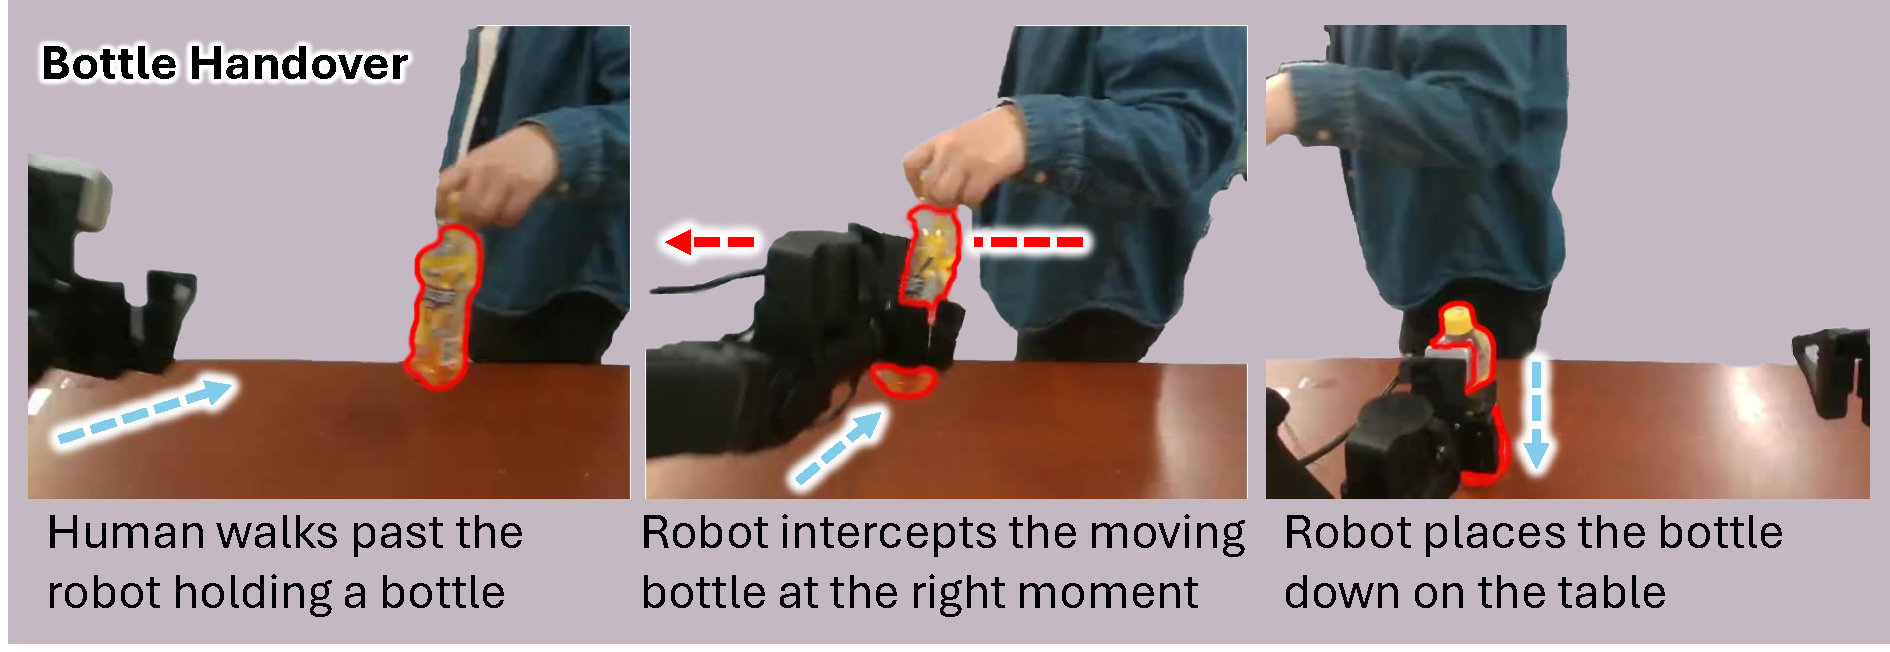
\includegraphics[width=0.5\columnwidth]{2026-corl-unveil-template/figures/handover.pdf}\hfill
	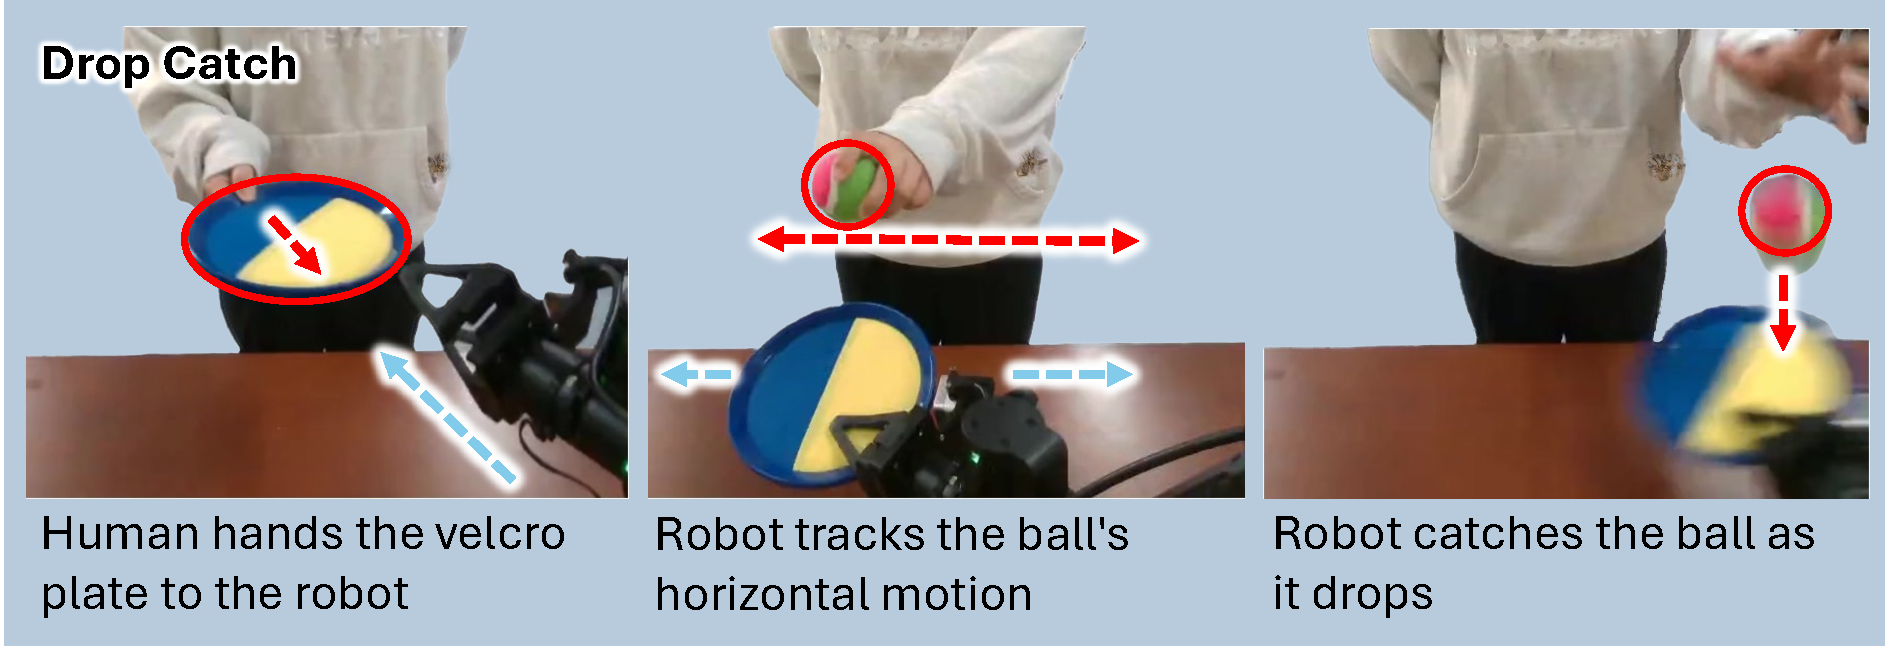
\includegraphics[width=0.5\columnwidth]{2026-corl-unveil-template/figures/drop.pdf}\\
	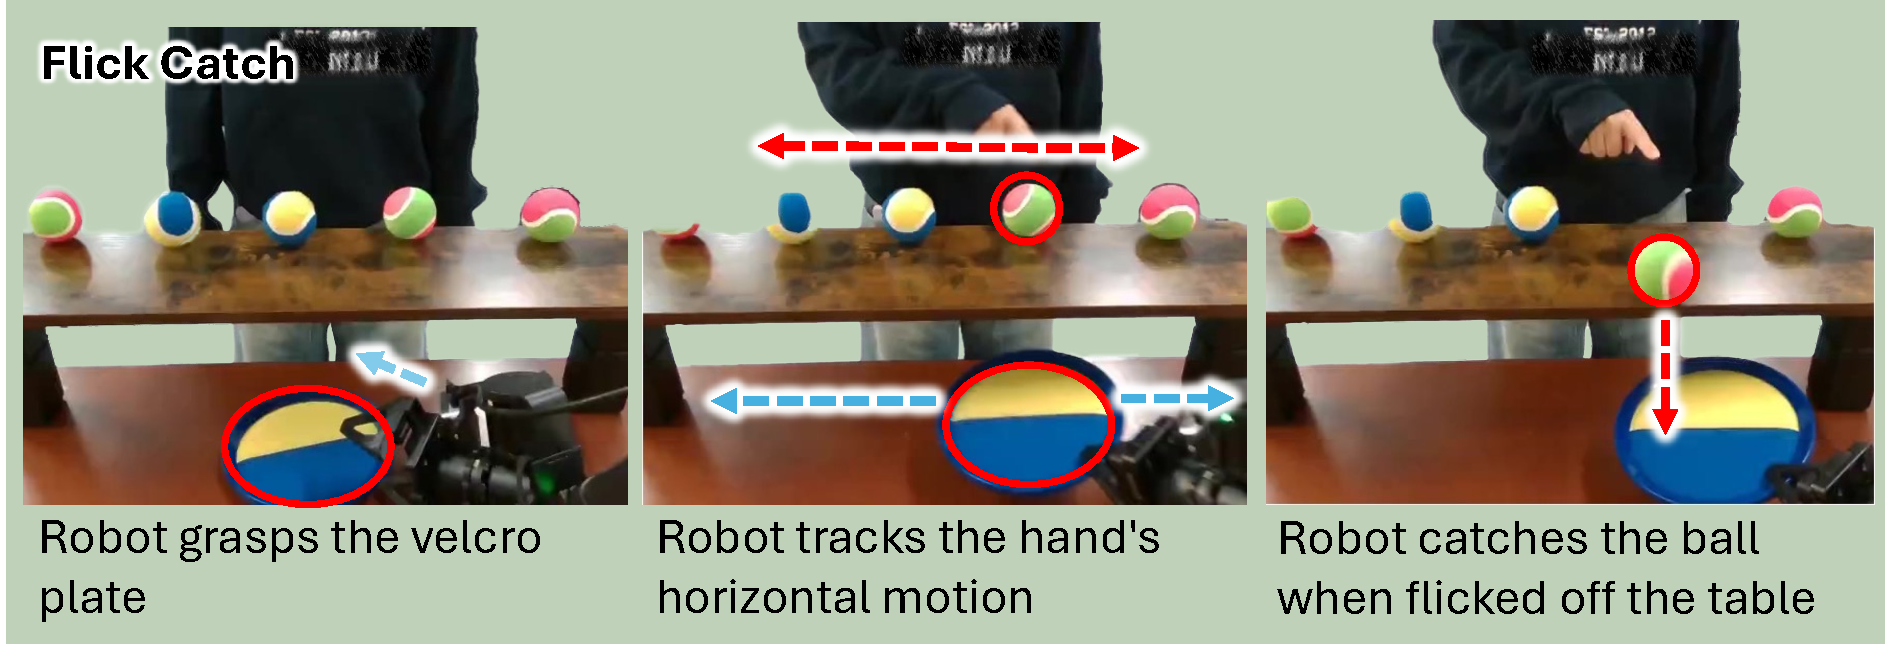
\includegraphics[width=0.5\columnwidth]{2026-corl-unveil-template/figures/flick.pdf}\hfill
	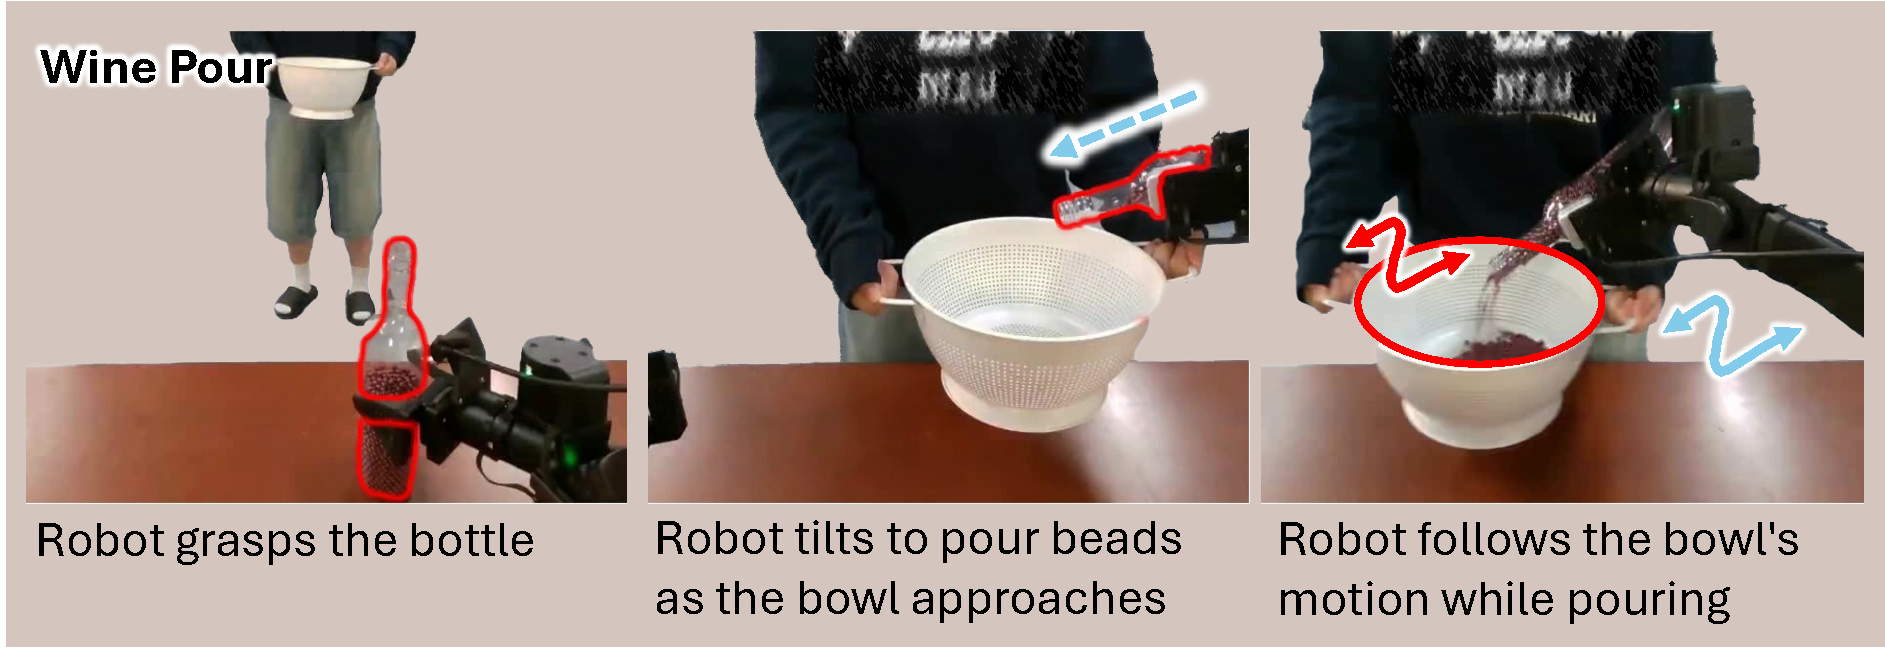
\includegraphics[width=0.5\columnwidth]{2026-corl-unveil-template/figures/pour.pdf}
	\caption{\textbf{Task Setup.} We benchmark all models across four comprehensive dynamic tasks.}
	\label{fig:tasks}
\end{figure}

We design four tasks to expose the two ambiguities identified in \cref{sec:introduction}: motion ambiguity and state aliasing. We ask whether \ours\ resolves each kind of ambiguity through \TEMPOMOT\ and \TEMPOACT. We compare \ours\ against two state-of-the-art asynchronous baselines designed for responsive task execution, RTC~\cite{rtc} and VLASH~\cite{vlash}. For Wine Pour and Flick Catch, both baselines collapse to $0\%$ on the full task because the release-and-retract phase is perceptually aliased with reaching. As a result, a baseline that sees the gripper near the bottle or plate cannot tell whether to grasp or withdraw and oscillates between the two (more detailed visualization and analysis in \cref{app:failure}). To avoid a trivial comparison, we report quantitative results on a trimmed version that removes the release-and-retract phase, eliminating this artifact. We emphasize that \ours\ disambiguates these phases through \TEMPOMOT\ and \TEMPOACT, so the gain in \cref{tab:success_rates} is a lower bound on \ours's full-task advantage. For qualitative rollouts of the baselines' complete failure and \ours's behavior, please see our project webpage and \cref{app:failure}.


\noindent\textbf{Task properties.}\label{sec:task_properties} Each of the four tasks is dynamic and shares four properties that a current-frame observation alone cannot resolve.
  \textbf{(P1)} The target object is moving at varying motion. Therefore, reacting based on the current snapshot alone is inaccurate in both position and timing.
  \textbf{(P2)} The relevant target shifts during the episode. As a result, the policy must redirect its attention to whichever object currently matters.
  \textbf{(P3)} Each task decomposes into a sequence of subtasks (approach, grasp, track, release), and the correct next action depends on which subtask has already been completed.
  \textbf{(P4)} The policy faces state ambiguity. From the current frame alone, multiple next actions are plausible, and a perceptually identical state may demand opposite actions depending on what has come before. 

   
\textbf{Bottle Handover (P1).}~The robot intercepts a bottle from a human walking by from either direction. We vary the walking speed, bottle's height, and holding pose across episodes, so the policy must estimate the bottle's velocity to time and place the grasp correctly.
\\\textbf{Drop Catch (P1, P3).}~The robot catches a ball dropped by a horizontally moving human hand. Each episode begins with the human handing a Velcro plate to the robot, after which the robot tracks the human’s hand laterally before catching the released ball. This task includes a moving dynamic object (P1) and multiple sequential subtasks (P3).
\\\textbf{Flick Catch (P1--P4).}~Several Velcro balls rest on a long horizontal platform. The robot first picks up a Velcro plate from the table (P3). A human hand then hovers over the balls and, at a random time, flicks one off the platform. The robot must first track the hand, then switch to tracking the released ball to catch it in time (P2, P1). Because the robot picks up and later places down the plate at the same location, the pick-up is perceptually aliased with the subsequent drop-off (P4), making this the most challenging of the four tasks.
\\\textbf{Wine Pour (P1--P4).}~The robot pours beads, an alternative to wine, into a pot that the human moves around. The task decomposes into three subtasks (P3): pick up the bottle from the table, pour while tracking the pot movement, and put the bottle back down. Pick-up and put-down produce visually similar states yet require opposite actions, producing state aliasing (P4). Once pouring begins, the target shifts from the bottle to the pot (P2), whose motion must be tracked (P1). Since every rollout inevitably spilled some beads, this task's success is determined by the percentage of beads' mass retained in the pot at the end of the pour.


\subsection{Experimental Results}
\label{sec:quant}

\begin{figure}[!tbp]
	\centering
 	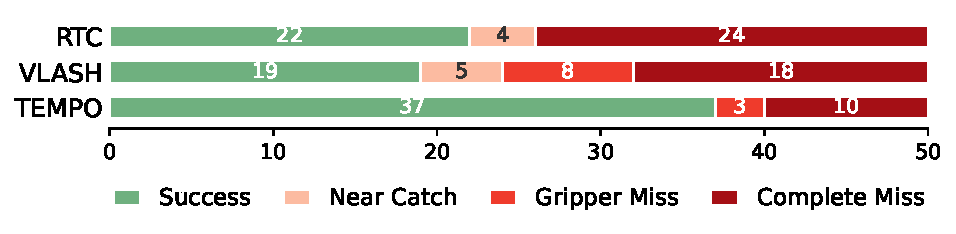
\includegraphics[width=0.8\columnwidth]{2026-corl-unveil-template/figures/failure_modes.pdf}
    \vspace{-1em}
	\caption{\textbf{Failure-mode breakdown on Bottle Handover}, we categorized and visually examined each episode in deployment rollouts and attributed each model's failure to different categories.}
	\label{fig:failure_modes}
\end{figure}

\noindent\textbf{Success Rate on Dynamic Tasks.}
As shown in \cref{tab:success_rates}, we extensively compare our method against each of the SOTA asynchronous VLA models. For each task, we calculated success rate for each model based on 50 trials following the evaluation protocol established under \cref{sec:setup}. On simpler tasks like Drop Catch, \ours\ achieves a competitive success rate compared to RTC, while VLASH frequently overshoots the human motion and misses the dropped ball. Across the remaining tasks where the object motion is more uncertain or the object of interest shifts, \ours\ consistently outperforms both baselines, including $+36\%$ on Bottle Handover, $+4.1\%$ on Wine Pour, and $+46\%$ on Flick Catch. We observed closer tracking of the human hand by the robot gripper in Drop Catch and Flick Catch, as well as more precisely timed grasps in Bottle Handover.




\noindent\textbf{Failure mode analysis.}
A single success rate hides \emph{why} a policy fails, so we visually examined all
$50$ rollouts of every model on Bottle Handover and labeled each as a success or
one of three failure modes (\figref{fig:failure_modes}). The dominant failure for both baselines is \emph{Complete Miss}, where the arm reaches toward the wrong place and misses the bottle entirely, indicating that the policy mispredicts where the moving bottle will be. VLASH and RTC commit $18$ and $24$ Complete Misses respectively, while the timing-related \emph{Gripper Miss} and the near-success \emph{Near Catch} are comparatively rare. By conditioning on recent motion, \ours\ cuts Complete Misses to $10$ and raises success from $19$ (VLASH) and $22$ (RTC) to $37$ out of $50$. Although both asynchronous pipelines significantly reduce inference delay, a lack of motion understanding still hurts dynamic-task performance.


\begin{wraptable}{r}{0.42\columnwidth}
\centering
\vspace{-\baselineskip}
\small
\setlength{\tabcolsep}{4pt}
\begin{tabular}{lcc}
\toprule
VLA backbone & Base & + \ours \\
\midrule
$\pi_{0.5}$~\cite{pi05}   & 26\% & \textbf{56\%} \\
RTC~\cite{rtc}            & 44\% & \textbf{80\%} \\
VLASH~\cite{vlash}        & 38\% & \textbf{74\%} \\
\bottomrule
\end{tabular}
\caption{\textbf{\ours\ is plug-and-play across VLA backbones.} Adding \TEMPOMOT\ and \TEMPOACT\ improves Bottle Handover on all backbones, including the non-asynchronous $\pi_{0.5}$.}
\label{tab:backbone_integration}
\end{wraptable}
\noindent\textbf{Plug-and-play across VLA backbones.}
The two temporal inputs of \ours\ are not backbone-specific. We attach the same \TEMPOMOT\ and \TEMPOACT\ to two additional pretrained VLAs, $\pi_{0.5}$~\cite{pi05} (non-asynchronous) and RTC~\cite{rtc}, and retrain each on the same Bottle Handover demos. Every backbone we tried improves substantially: $\pi_{0.5}$ from $26\%$ to $56\%$, RTC from $44\%$ to $80\%$, and VLASH from $38\%$ to $74\%$ (\cref{tab:backbone_integration}). \ours\ helps both asynchronous and non-asynchronous backbones, indicating that motion-aware perception is a general upgrade rather than a VLASH-specific effect.


\noindent\textbf{Extending TEMPO with a compact training target.}
With \ours\ closing the input-side gap, a natural line of question being whether anything remains on the output side. Our prior work, Unified Visuomotor Target (UVT)~\cite{uvt}, argues that it does: VLAs are typically trained to predict raw joint-position chunks, which are high-dimensional and jitter-prone, and swapping this target for a compact motion primitive aligned with object motion tightens the target the policy has to learn. Since \ours\ and UVT act on different sides of the policy, they combine without redundancy: \ours+UVT achieves the highest overall success rate in \cref{tab:success_rates} and outperforms baselines on $3$ of the $4$ tasks, further pushing dynamic task performances.


\section{Analysis and Ablations}
\label{sec:ablation}
% Commented out: fig:attention (attention-mass visualization). The
% qualitative attention story was largely a narration of the figure
% and correlational; the causal input-ablation MSE curves in
% app:input_ablation carry the 'each signal matters at a different
% moment' claim more sharply.
\iffalse
\begin{figure}[t]
	\centering
	\includegraphics[width=0.8\columnwidth]{2026-corl-unveil-template/figures/attention_shrink.pdf}
	\vspace{-1em}
    \caption{\textbf{The policy attends to \TEMPOMOT\ and \TEMPOACT\ at different stages of the task.} \TEMPOMOT\ attention peaks when the human hand starts moving, whereas \TEMPOACT\ attention peaks during fast hand following.}
	\label{fig:attention}
\end{figure}
\fi



% Having shown that \ours\ outperforms recent VLA baselines on dynamic tasks that target execution latency rather than motion perception (\tabref{tab:success_rates}), we now turn to \emph{why}. Here we show that conditioning on two signals, the global object motion~(\TEMPOMOT) and the robot's joint history~(\TEMPOACT), is crucial for addressing two ambiguities: motion and state.

% We analyze along three axes.
% To show that both \TEMPOMOT~and \TEMPOACT~ are crucial for dynamic tasks, we propose three questions:
  % \textbf{(i) Why these two signals?} The structure of dynamic tasks that \TEMPOMOT\ and \TEMPOACT\ carry information that the current frame alone cannot provide.
  % \textbf{(ii) How does the policy uses both signals?} Action Expert (AE) transformer attention mass (\figref{fig:attention}) and per-frame ablation MSE (\figref{fig:attention_mse}) shows that \ours\ relies on \TEMPOMOT\ and \TEMPOACT\ at different moments, and that removing either causes the policy to revert to jittery and reactive behavior (\figref{fig:jittery}).  
  % \textbf{(iii) But what does \TEMPOMOT\ actually encode?}A linear probe of \TEMPOMOT\ against \llm{semi-automated annotation of object velocity} confirms that object motion is represented in the token.


Having shown \ours\ outperforms recent VLA baselines on dynamic tasks, we now turn to \emph{why}. We evaluate whether the policy relies on \TEMPOMOT\ and \TEMPOACT\ at the task stages where their corresponding ambiguities arise, using single-signal ablations and hidden-state probing.

% Commented out: attention-mass paragraph accompanying fig:attention.
% It was largely a narration of the figure and did not add a claim
% beyond what tab:input_ablation and app:input_ablation already carry.
\iffalse
In \figref{fig:attention}, we visualize how strongly the action expert emphasizes the two temporal signals over time. We investigate a representative episode on one of our hardest tasks, Flick Catch, and plot the attention mass that our model places on \TEMPOMOT\ and \TEMPOACT\ over the course of the episode. The \TEMPOMOT\ signal is emphasized as the human hand starts moving, which corresponds to major movement in the observation. \TEMPOACT\ then steadily gains more attention mass during the hand-following phase and drops back down after the ball is successfully caught. The same pattern generalizes across rollouts. Dropping \TEMPOMOT\ or \TEMPOACT\ during important phases significantly degrades action quality; see \cref{app:input_ablation} for the full ablation analysis.
\fi

  % Having motivated the design, we now show that the policy especially relies on \TEMPOMOT\ and \TEMPOACT~at certain crucial moments for the task. To verify, we examine when the policy attends to each signal and whether the two signals carry separable information by investigating what happens if we remove them.


\begin{wraptable}{r}{0.38\columnwidth}
\centering
\vspace{-\baselineskip}
\small
\setlength{\tabcolsep}{4pt}
\begin{tabular}{lc}
\toprule
Configuration & Handover \\
\midrule
\TEMPOACT\ only & 52\% \\
\TEMPOMOT\ only & 56\% \\
\ours\ (full)   & \textbf{74\%} \\
\bottomrule
\end{tabular}
\caption{\textbf{Both temporal signals contribute to the task.} Removing either \TEMPOMOT\ or \TEMPOACT\ reduces Bottle Handover success; the two together outperform either alone.}
\label{tab:input_ablation}
\end{wraptable}
\noindent\textbf{Each temporal signal is individually necessary.}
To verify that both \TEMPOMOT\ and \TEMPOACT\ carry non-redundant information for task success, we retrain \ours\ with each single signal removed and evaluate on Bottle Handover (\cref{tab:input_ablation}). Removing either signal substantially reduces success, and both single-signal variants still outperform the VLASH baseline (38\%), confirming that each temporal input is independently useful. Combining the two lifts success to $74\%$, above what either signal alone achieves. Each signal is also consulted at a distinct moment in the episode; see \cref{app:input_ablation} for the per-frame ablation MSE.


\noindent\textbf{Baseline hidden states lack motion on the hardest tasks.}
\label{para:motion_probe}
We test whether the trained policy encodes object motion by probing its hidden state at a fixed token position, following the same protocol as prior VLM probe works~\cite{zhao2024first, lu2025probing}. For each task we annotate the per-frame position of the object of interest and compute its pixel-space velocity, yielding an object-motion benchmark of over 50k annotated frames of human-robot dynamic manipulation that we release as \benchname, together with a multiple-choice variant in the format of MVBench~\cite{li2024mvbench} and VLM4D~\cite{zhou2025vlm4d}. Here we report the regression setting: we fit an MLP probe from each model's hidden state to the velocity and report $R^2$ (\cref{tab:motion_probe}).

\ours\ produces the strongest probe result on every row of \cref{tab:motion_probe}. Its hidden state decodes object velocity substantially better than the asynchronous baselines on the dynamic tasks where motion is the only cue (Flick Catch $R^2 = 0.57$ vs.\ ${\le}\,0.03$; Wine Pour $R^2 = 0.44$ vs.\ ${\le}\,0.09$), where the baseline probes collapse to near zero. Since RTC, VLASH, and \ours\ share the same $\pi_{0.5}$ backbone and pretraining, \ours's gain over the two is attributed to its motion-conditioned fine-tuning: \TEMPOMOT\ and \TEMPOACT\ leave a linearly-decodable motion signal in the hidden state that the other $\pi_{0.5}$-family backbones do not carry. We additionally ablate the choice of motion encoder, probing several video foundation models' latents for object velocity, in \cref{app:motion_encoder}.

\begin{table}[!t]
\centering
\small
\begin{tabular}{lccc}
\toprule
Task & RTC~\cite{rtc} & VLASH~\cite{vlash} & \ours \\
\midrule
Bottle Handover  & 0.46 & 0.43 & \textbf{0.52} \\
Drop Catch       & 0.31 & 0.28 & \textbf{0.33} \\
Flick Catch      & $-0.07$ & 0.03 & \textbf{0.57} \\
Wine Pour        & 0.06 & 0.09 & \textbf{0.44} \\
\midrule
Average          & 0.19 & 0.21 & \textbf{0.47} \\
\bottomrule
\end{tabular}
\vspace{1em}
\caption{\textbf{Motion probing of the trained VLA hidden state.} MLP probe on object velocity across our dynamic tasks ($R^2$). On Flick Catch and Wine Pour, where motion is the only usable cue, the asynchronous baselines' representations collapse to near zero while \ours's remains informative.}
\label{tab:motion_probe}
\vspace{-1em}
\end{table}

\label{sec:analysis}


%===============================================================================
